\documentclass[oneside,10pt]{article}
\usepackage[latin1]{inputenc}
\usepackage[francais]{babel}
\usepackage[francais]{layout}
\usepackage[OT1]{fontenc}
\usepackage{listings}
\usepackage{cite}
\usepackage{textcomp}
\usepackage{graphicx}

% Reglages du document
\lstset{language=bash, frame=single, breaklines=true, basicstyle=\ttfamily, keywordstyle=\bfseries}
\setlength{\hoffset}{-18pt}        
\setlength{\oddsidemargin}{0pt} % Marge gauche sur pages impaires
\setlength{\evensidemargin}{9pt} % Marge gauche sur pages paires
\setlength{\marginparwidth}{54pt} % Largeur de note dans la marge
\setlength{\textwidth}{481pt} % Largeur de la zone de texte (17cm)
\setlength{\voffset}{-18pt} % Bon pour DOS
\setlength{\marginparsep}{7pt} % S�paration de la marge
\setlength{\topmargin}{0pt} % Pas de marge en haut
\setlength{\headheight}{13pt} % Haut de page
\setlength{\headsep}{10pt} % Entre le haut de page et le texte
\setlength{\footskip}{27pt} % Bas de page + s�paration
\setlength{\textheight}{708pt} % Hauteur de la zone de texte (25cm)

\begin{document}

% Page de couverture
\title{Proposition de solution : ch\`eque num\'erique, version shell}
\author{Louis BILLIET \\ Florent DAVID}
\date{25 Sept. 2013}
\maketitle

\section{Changements techniques}
Dans la version \'ecrite en python de notre ch\'equier, nous utilisions le chiffrement par RSA pour s'assurer qu'un message soit bien \'emit par la personne avec laquelle on discute.
Nous pouvions donc communiquer librement les ``cl\'es publiques'' afin de d\'echiffrer ces messages.
Dans la philosophie d'OpenSSL, le chiffrement sert \`a emp\^echer un tiers de lire un message s'il ne lui est pas address\'e.
Pour assurer l'int\'egrit\'e d'un message, nous devons d\'esormais passer par la signature.


Donc, au lieu de chiffrer compl\`etement un message, nous archivons diff\'erents fichiers avec leurs hach\'es sign\'es.
Cela acc\'el\`ere le traitement et diminue la taille des messages.
Par contre, l'arborescence des fichiers est devenue quelque peu complexe.
Nous traiterons des d\'etails de cette arborescence dans le dernier chapitre.

\section{Pr\'eparations avant ex\'ecution}
Pour une execution sans accrocs des differents scripts, il faut que l'entit\'e ``banque'' existe avec ses differents fichiers de persistence :
\begin{verbatim}
mkdir banque
sh GenererCles.sh 2048 banque
touch banque/ribsFile
\end{verbatim}

\section{Trace d'execution}
Voici une trace d'ex\'ecution type. En cas de doute, vous pouvez invoquer les scripts sans arguments pour connaitre l'usage.
\begin{verbatim}
$ # Creation d'un dossier par acteur. Victor est le vendeur et Charles, le client
$ mkdir Victor Charles
$ # Generation des cles RSA des acteurs
$ sh GenererCles.sh 512 Victor
$ sh GenererCles.sh 512 Charles
$ # Generation des certificats de la banque
$ sh GenererCertif.sh Victor
$ sh GenererCertif.sh Charles
$ # Creation d'une facture
$ sh CreerFacture.sh 10.00 Victor
$ # Creation d'un cheque
$ sh CreerCheque.sh Victor/facture1.tgz Charles
voulez-vous payer 10.00 euros a Victor ? (oui/non) non
paiement annule
$ sh CreerCheque.sh Victor/facture1.tgz Charles
voulez-vous payer 10.00 euros a Victor ? (oui/non) oui
$ # Verification de cheque par le vendeur
$ sh VendeurVerifieCheque.sh Victor/facture1.tgz Charles/cheque3927128561.tgz
Seems legit.
$ # Verification du cheque par la banque
$ sh BanqueVerifieCheque.sh Charles/cheque3927128561.tgz
Seems legit.
\end{verbatim}
Attention !
Certains arguments sont des fichiers g\'en\'er\'es par les scripts : les fichiers de facture (\verb+Victor/facture1.tgz+) et de ch\`eque (\verb+Charles/cheque3927128561.tgz+).
Ces fichiers sont g\'en\'er\'es selon la forme suivante : 
\begin{itemize}
\item facture : \textless Acteur\textgreater/facture\textless num\'ero de transaction\textgreater.tgz
\item ch\`eque : \textless Acteur\textgreater/cheque\textless RIB acteur\textgreater \textless num\'ero de transaction\textgreater.tgz
\end{itemize}

\section{Arborescence de fichiers}
\subsection{Les certificats d\'elivr\'e par la banque}
Le but du certificat d\'elivr\'e par la banque est d'avoir une preuve d'authenticit\'e du compte de l'acteur qui le d\'elivrera.
Pour cela il contient 3 \'el\'ement:
\begin{itemize}
\item Le certificat en clair (qui mentionne en 3 lignes: Nom, N� de compte et la cl\'e public du propri\'etaire de ce compte)
\item Le hash\'e-chiffr\'e du certificat
\item La cl\'e public de la banque pour lire le hash\'e et v\'erifier l'authenticit\'e du banque.certif
\end{itemize}
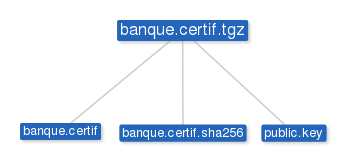
\includegraphics[scale=0.75]{banque_certif.jpg}

\subsection{La facture}
La facture est repr\'esent\'e par une archive qui contient les \'el\'ement suivant:
\begin{itemize}
\item La facture en clair (qui mentionne en 2 lignes: montant et N� de facture)
\item Le hash\'e-chiffr\'e de la facture
\item L'archive banque.certif.tgz qui a \'et\'e d\'elivr\'e par la banque, pour que le client aie les coordon\'e banquaire du vendeur.
\end{itemize}
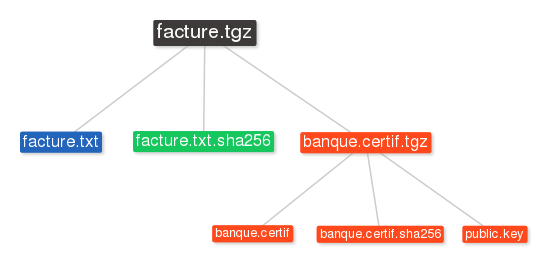
\includegraphics[scale=0.75]{facture_archi.jpg}

\subsection{Le cheque}
Le cheque est repr\'esent\'e par une archive qui contient les \'el\'ement suivant:
\begin{itemize}
\item Le cheque en clair (qui mentionne en 3 lignes: le rib du vendeur, le montant et le N� de facture)
\item Le hash\'e-chiffr\'e du cheque
\item L'archive banque.certif.tgz qui a \'et\'e d\'elivr\'e par la banque, pour que le vendeur aie les coordon\'e banquaire du client.
\end{itemize}
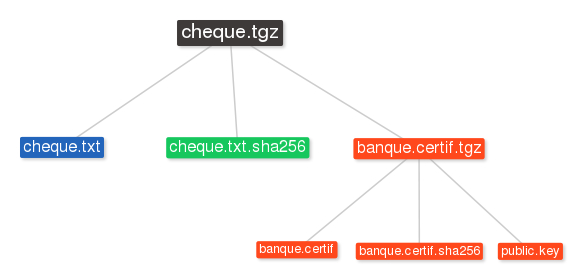
\includegraphics[scale=0.75]{cheque_archi.jpg}

\end{document}
